% Második előadás

\chapter{Mobil és táblagép processzorok fejlődése}

\section{Bevezetés}
Az okostelefonok 2006 körül jelentek meg, a táblagépek ennél is később, 2010-ben.
A fő prioritás az üzemidő, tehát alacsony fogyasztású processzorokat kell fejleszteni.
Ez ellentétes az addig uralkodó fejlesztési iránytól (legnagyobb teljesítmény wattonként).

\section{Fogyasztás csökkentése}
Az alacsony fogyasztást kétféleképpen lehet elérni:
\begin{itemize}
    \item keskeny mikroarchitektúrákkal
    \item alacsony órafrekvenciával.
\end{itemize}

Az ARM Cortex család korai tagjai ezt általában 2 (3 a Cortex A15 esetében) széles architektúrával (egyszerre 2 utasítás vágrehajtására képes) érték el.

\subsection{Intel Atom}
Az Intel viszont a Core 2 családtól kezdve 4 szélességű architektúrát implementált, a nagyobb teljesítmény/fogyasztás arány elérése érdekében.
Következmény, hogy az Intel és AMD hagyományos mikroarchitektúrái nem voltak versenyképesek az ARM-el szemben.
Ezért kifejlesztettek egy új mikroarchitektúrát, ami 2 szélességű.
Így jött létre 2008-ban az Intel Atom családja, amire alapozva megjelentek az Intel okostelefon platformjai.

\subsection{AMD}
2011 környékén az AMD a Bulldozer mikroarchitektúrára épülő processzorokat gyártotta, ami végül nem vált be.
Ezzel párhuzamosan bevezették a kisebb fogyasztású Cat mikroarchitektúrát, az Atomhoz hasonlóan 2 szélességgel.
Ez is a mobil piacot célozta.

\subsection{A frekvencia csökkentése}
A disszipáció két részből áll: statikus és dinamikus.
Statikus a zárt tranzisztorokan szivárgó áram által keltett disszipáció, dinamikus pedig a működő tranzisztorok által keltett.
Következmény, hogy a dinamikus disszipáció egyenesen arányos az órafrekvenciával, mivel magasabb frekvencián több töltés-kisülés keletkezik.
Ezen kívül négyzetesen arányos a magfeszültséggel (Ohm-törvény).
Tehát a dinamikus disszipáció:
\begin{equation}
    D_d = const * f_c * V^2
\end{equation}
Mivel a frekvenciához arányosan nagyobb feszültség kell, ezért a disszipáció a frekvencia növelésével köbösen növekszik.
Ezt mutatja a \ref{fig:skylake}. ábra.
\begin{figure}[H]
    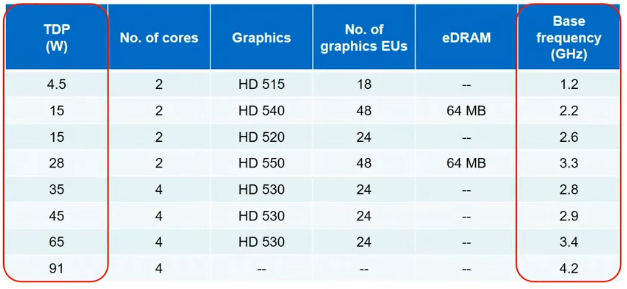
\includegraphics[width=0.8\textwidth]{skylake}
    \centering
    \caption{Az Intel Skylake család órajelei és fogyasztásai}
    \label{fig:skylake}
\end{figure}

A Skylake család gyengébb tagjait táblagépekbe szánták, ezeknél az alacsony fogyasztás érdekében gyengébb grafikát, kevesebb magot és alacsony órajelet használtak.

\section{Piaci részesedés}
A fejlesztések ellenére az Intelnek és AMD-nek nem sikerült betörniük a mobil eszközök piacára.

\begin{figure}[H]
    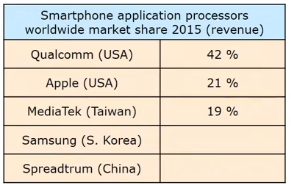
\includegraphics[width=0.8\textwidth]{market}
    \centering
    \caption{Az okostelefon processzorok piaci részesedése 2015-ben}
    \label{fig:market}
\end{figure}

Bár az Intel a táblagépeknél elért valamekkora részesedést, ezt úgy érte el, hogy fizetett a gyártóknak az Atom processzor használatáért.

\begin{figure}[H]
    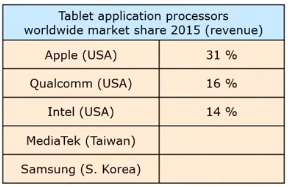
\includegraphics[width=0.8\textwidth]{markettablet}
    \centering
    \caption{A táblagép processzorok piaci részesedése 2015-ben}
    \label{fig:markettablet}
\end{figure}

A gyártóknak fizetett összegek miatt az Intelnek 2 év alatt 7 milliárd dollár vesztesége keletkezett.
A nagy veszteségek miatt 2016-ban az Intel visszavonult a mobil piacról, a már bejelentett rendszereket pedig törölték.
Ezzel együtt 12000 embert bocsátottak el.

Az AMD 2015-ban még megjelentetett egy új mobil családot, de a 2016-os kínálatban már nem szerepeltek mobil processzorok.
Helyette 2017-től a Zen architektúrát fejlesztették.

Az Nvidia szintén gyártott mobil processzorokat a 2010-es évek elején, de 2016-ban ők is kivonultak a piacról.

\section{Szélesség fejlődése}
A keskeny szélesség és alacsony frekvencia követelmények a processzorok fejlődésével kevésbé lettk lényegesek, mivel nagyon sok fejlesztés történt a disszipáció csökkentésére.
2010 környékén még jellemzően 2 széles rendszerek voltak a mobilokban, aztán a teljesítmény növelése érdekében 3 szélesre növelte a processzorait az ARM, az Apple, a Qualcomm és a Samsung is.
A fejlődés itt nem állt meg, az ARM 2018-ban 4 széles rendszereket hozott ki.
Szintén 4 széles a Samsung M1 magja is.
Ezután még 6, 7 és 8 széles architektúrákat is bejelentettek.
Az Apple pl. nagyon korán (2013-ban) 6 széles magot mutatott be (Jim Keller fejlesztése).